\documentclass[tikz,border=12pt]{standalone}
\usepackage{amsmath,amssymb}
\usepackage{tikz}
\usetikzlibrary{arrows.meta,positioning,fit,calc,backgrounds}
\tikzset{
  box/.style={
    draw,
    very thick,
    rectangle,
    align=center,
    inner sep=8pt,
    minimum height=1.25cm,
    minimum width=3.1cm,
    font=\small,
  },
  wide/.style={box, minimum width=3.6cm},
  arr/.style={-{Stealth[length=2.6mm, width=2mm]}, thick},
  barr/.style={
    {Stealth[length=2.4mm, width=1.8mm]}-{Stealth[length=2.4mm, width=1.8mm]},
    thick,
  },
  lbl/.style={font=\scriptsize, inner sep=2pt, fill=white},
  group/.style={draw, dashed, inner sep=12pt},
}

\begin{document}
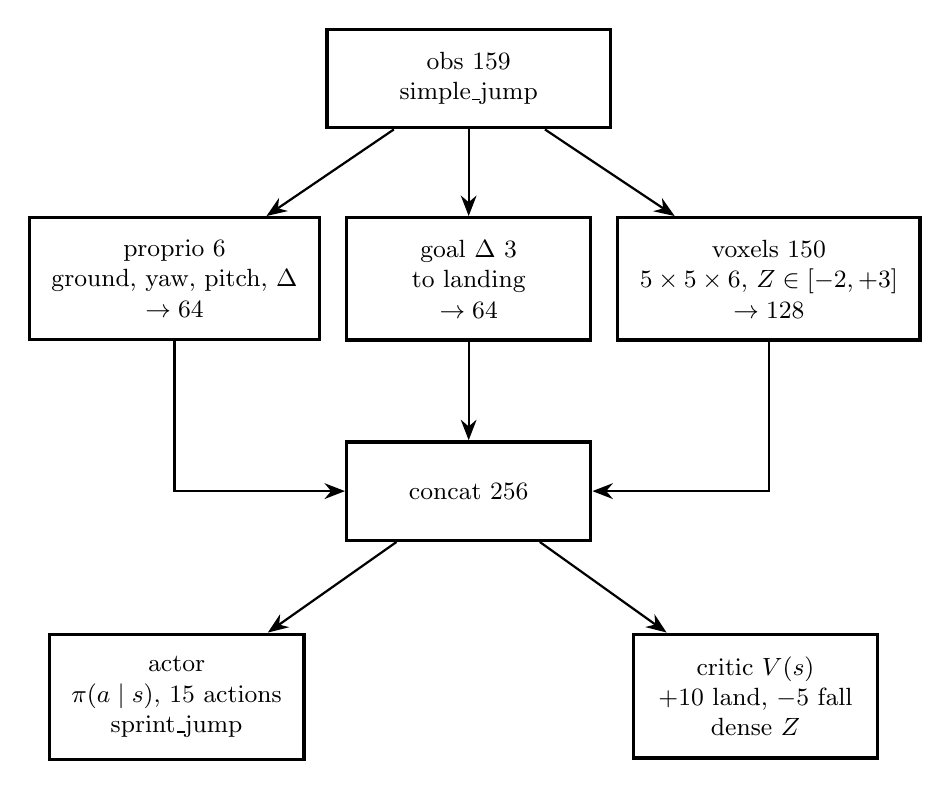
\begin{tikzpicture}[node distance=0.8cm and 0.65cm]
  \node[wide] (obs) {obs $159$\\simple\_jump};

  \node[box, below left=1.1cm and 0.05cm of obs] (p) {proprio $6$\\ground, yaw, pitch, $\Delta$\\$\to 64$};
  \node[box, below=1.1cm of obs] (g) {goal $\Delta$ $3$\\to landing\\$\to 64$};
  \node[box, below right=1.1cm and 0.05cm of obs] (v) {voxels $150$\\$5\times5\times6$, $Z\in[-2,+3]$\\$\to 128$};

  \node[box, below=1.25cm of g] (cat) {concat $256$};

  \node[box, below left=1.15cm and 0.5cm of cat] (act) {actor\\$\pi(a\mid s)$, $15$ actions\\sprint\_jump};
  \node[box, below right=1.15cm and 0.5cm of cat] (crt) {critic $V(s)$\\$+10$ land, $-5$ fall\\dense $Z$};

  \draw[arr] (obs) -- (p);
  \draw[arr] (obs) -- (g);
  \draw[arr] (obs) -- (v);
  \draw[arr] (p) |- (cat);
  \draw[arr] (g) -- (cat);
  \draw[arr] (v) |- (cat);
  \draw[arr] (cat) -- (act);
  \draw[arr] (cat) -- (crt);
\end{tikzpicture}
\end{document}
